\documentclass{article}
\usepackage{graphicx}
\usepackage{bm}
\usepackage{datetime2}
\usepackage{amsmath}
\usepackage{amssymb}
%\usepackage{unicode-math}
\usepackage{amsfonts} 
\usepackage{afterpage}
\usepackage{indentfirst}
\usepackage[margin=1in]{geometry} 
\usepackage{nameref}
\usepackage{booktabs}
\usepackage{latexsym}
\numberwithin{equation}{section}
\numberwithin{figure}{section}
\usepackage{caption}
\usepackage{float}
\usepackage{color}



\title{ Steady State Lid Driven Cavity Using Simple Algorithm - Finite Volume Method}
\author{Ganesh Borde}
\date{December 2024}
\begin{document}
\maketitle
\begin{abstract}
    This project focuses on the numerical simulation of flow inside a two-dimensional lid-driven 
    cavity. The study investigates the flow properties at low Reynolds numbers to 
    achieve a steady-state solution. A pressure correction approach, specifically the 
    Semi-Implicit Method for Pressure Linked Equations (SIMPLE), is employed to solve 
    the incompressible Navier-Stokes equations. The finite volume  discretization (FVM) 
    method is used. The numerical results are validated against benchmark solutions of 
    cavity flow reported in the literature. Various flow characteristics and results 
    are analyzed in detail.
\end{abstract}
\section{Introduction}
The lid-driven cavity is a benchmark problem in the study of Computational 
Fluid Dynamics (CFD). Its simplicity allows researchers to evaluate the accuracy and 
stability of numerical methods. This problem has been extensively studied for over 50 years. Let 
us discuss about the problem below.

\subsection{Problem description}
The lid-driven cavity is a two-dimensional domain bounded by three stationary walls and one 
moving boundary, i.e., the top wall moving with a velocity \( U \), as shown in Fig.~\ref{fig:lid_driven}. The 
cavity is considered a square domain, where the length of all sides is \( L \). As the 
top wall moves with a velocity \( U \), the flow inside the cavity experiences motion 
due to the viscous nature of the fluid. 

The velocity values at the three fixed boundaries are \( u = v = 0 \), while the 
moving boundary has \( u = U \) and \( v = 0 \). In this project, the cavity is 
studied by setting the velocity \( U = 1 \, \mathrm{m/s} \) and the length of 
the boundary \( L = 1 \, \mathrm{m} \). Only the viscosity of the flow is 
varied, while the density of the flow is kept constant. The flow properties are analyzed 
for different viscosities. The pressure fields are not included in the results section, as 
their sole purpose in this study is to project the velocity field onto the solenoidal space.

\begin{figure}[t]
    \centering
    \label{fig:lid_driven}
    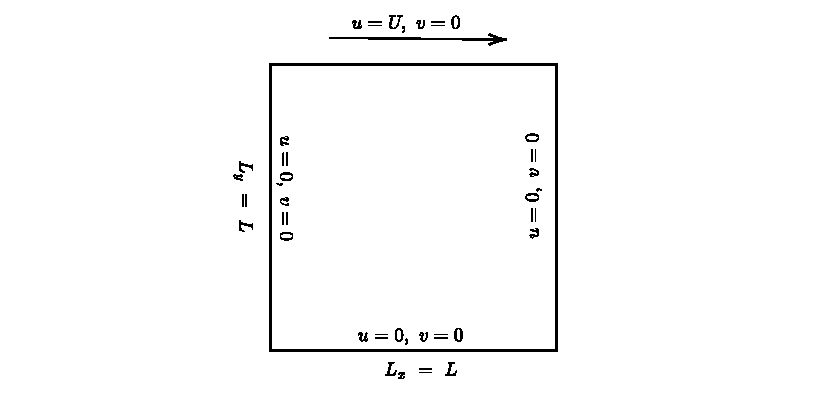
\includegraphics{lid_driven.pdf}
    \caption{Problem description of lid-driven cavity flow.}
\end{figure}

\subsection{Governing equations}
As mentioned, the flow is steady, incompressible, two-dimensional and isothermal. Therefore, 
the 2-D incompressible Navier-Stokes equations are considered, which are divided 
into the continuity equation, x-momentum equation, and y-momentum equation.

After non-dimensioning the variables as:
\begin{itemize}
    \item Length scale $x = \overline{x} L$ and $y = \overline{y} L$  
    \item  Velocity scale $u =\overline{u} U$ and $v =\overline{v} U$
    \item Pressure $p=\overline{p}\rho U^2$
\end{itemize}
The resulting governing  equations (omitting the bar notations for the sake of simplicity) are:
\begin{equation}
    \frac{\partial u}{\partial x} + \frac{\partial v}{\partial y} =0,
    \label{eq:con}
\end{equation}
\begin{equation}
    \label{Eq:x_mom}
    \frac{\partial u u}{\partial x} + \frac{\partial u v}{\partial y} = - \frac{dp}{dx}+\frac{1}{\text{Re}}  \left [ \frac{\partial^2 u}{\partial x^2} + \frac{\partial^2 u}{\partial y^2}\right ],
\end{equation}
\begin{equation}
    \label{Eq:y_mom}
    \frac{\partial u v}{\partial x} + \frac{\partial v v}{\partial y} = - \frac{dp}{dy}+\frac{1}{\text{Re}}  \left [ \frac{\partial^2 v}{\partial x^2} + \frac{\partial^2 v}{\partial y^2}\right ].
\end{equation}
In Eq.~\ref{Eq:x_mom} and \ref{Eq:y_mom}, Re is reynolds number of the flow, defined as:
\begin{equation}
    \text{Re}= \frac{\rho U L}{\mu},
\end{equation}
where $\mu$ is the viscosity of the fluid.

\subsection{Literature review}
Lid-driven cavity flow problem is a test case type problem for 
incompressible solvers. The past work done on lid-driven cavity 
flow gives a range for steady solution. For a wide range of 
Reynolds numbers, Shen \cite{shen1991hopf} examined the flow structures in a 
unit cavity and discovered that the flow establishes a steady 
character for Re 10000.

The difference between the projection method and the SIMPLE method 
is the projection method is generally second-order accurate, which 
is developed for the simulation of incompressible unsteady flows 
by employing a non-linear update of pressure term, which may depend 
on the grid size, time step, and even velocity. It has three and 
four-step projection method. One of the famous methods by 
Chorin~.\cite{chorin1997numerical}.The standard SIMPLE method is written 
in a concise formula for steady and unsteady flow. It is proven that SIMPLE 
type methods have second-order temporal accuracy for unsteady flows. The 
classical second-order projection method and SIMPLE type methods are 
united within the framework of the general second-order projection formula \cite{ni2007bridge}. 


\section{Numerical method}
This section deals with the numerical method, discretization, and grid approach in solving 
the lid-driven cavity. The SIMPLE algorithm on the staggered grid configuration 
is used. First, let’s talk about the staggered grid. 
\subsection{Staggered grid}
A staggered grid is a configuration used for spatial discretization. Scalar 
variables (such as pressure \( p \), density \( \rho \), total enthalpy \( h \), etc.) 
are stored at the cell centers of control volumes, whereas velocity components (such as 
\( u \) and \( v \)) or momentum variables are stored at the cell faces. This configuration 
differs from a collocated grid, where all variables are stored at the same locations. For 
compressible or incompressible flow simulations using structured grids, staggered storage is primarily utilized.

Collocated grids are prone to a discretization error known as odd-even 
decoupling, which leads to checkerboard oscillation patterns in the solutions. By 
using a staggered grid, odd-even decoupling between pressure and velocity can be 
effectively avoided. In a staggered grid, pressure values (\( p \)) are located at the 
center of the cells, while the velocity components \( u \) and \( v \) are stored at the cell 
faces, as shown in Fig.~\ref{}.
\begin{figure}
    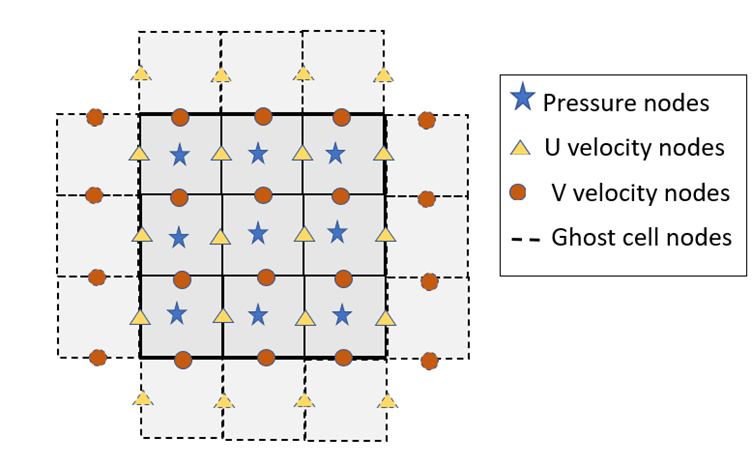
\includegraphics{staggered_grid.png}
    \caption{Staggered grid configuration}
\end{figure}

Boundary conditions can be defined in two different forms: 
Dirichlet boundary condition, where primary variables are specified, and 
Neumann boundary condition, where derivatives, such as pressure gradients, are specified. 

To apply boundary conditions, ghost cells (cells beyond the actual computational domain) 
are introduced. Ghost cells in the \( x \)-direction are represented by dashed lines, 
which indicate the \( v \)-velocity, while those in the \( y \)-direction represent 
the \( u \)-velocity. Pressure nodes are considered in both the \( x \)- and \( y \)-
directions. The updated number of variables in the system is presented in Table~\ref{tab:variables}.

\begin{table}
    \centering
    \caption{The number of variables in the domain}
    \label{tab:variables}
    \begin{tabular}{c c c}
        \toprule
        Field quantity & Interior resolution   & Resolution with boundary points \\
        \midrule
        $p$             & $n_x \times n_y$      & $(n_x +2)\times(n_y +2)$         \\
        $u$             & $(n_x -1) \times n_y$ & $(n_x+1)\times(n_y +2) $        \\
        $v$             & $n_x \times (n_y -1)$ & $(n_x +2)\times(n_y +1)$         \\
        \bottomrule        
    \end{tabular}
\end{table}

\subsection{Discretization}
The governing equations are discretized using finite volume method. The velocity at cell center p, is approximated 
by cell centers of east e, west w, north n, and south s. The $u$ and $v$  are indexing at $(i,j)$ (they are not on same point, because they have meshes for each other) and $p$  at $(I,J)$. So, the $x$ momentum 
equation (Eq.~\ref{Eq:x_mom}) can be approximated as
\begin{equation}
    \label{eq:x_mom_2}
    \frac{(u \hat{u})_e -(u \hat{u})_w}{\Delta x}+\frac{(u \hat{v})_n -(u \hat{v})_s}{\Delta y}
    = -\frac{p_{I+1,j}-p_{I-1,j}}{\Delta x}  +  \frac{1}{Re} \left [\frac{u_{i-1,j}-2u_{i,j}+u_{i+1,j}}{(\Delta x)^2} + \frac{u_{i,j-1}-2u_{i,j}+u_{i,j=1}}{(\Delta y)^2}\right ],
\end{equation}
where the $u, v$ velocities at each cell centers as
\begin{equation}
    v_n = \frac{v_{i,j}+v_{i+1,j}}{2}, v_s = \frac{v_{i,j-1}+v_{i+1,j-1}}{2},
    \label{eq:x_u_v1}
\end{equation}
and
\begin{equation}
    u_e = \frac{u_{i,j}+u_{i+1,j}}{2}, u_w = \frac{u_{i,j}+u_{i-1,j}}{2}, u_n = \frac{u_{i,j}+u_{i,j+1}}{2}, u_s = \frac{u_{i,j}+u_{i,j-1}}{2}.
    \label{eq:x_u_v2}
\end{equation}
In Eq.~\ref{eq:x_mom_2} $\Delta x$ and $\Delta y$ is the grid spacing in x and y direction respectively. This equation can be written as systems of equations as
\begin{equation}
    a_p u_{i,j} = a_e u_{i+1,j} + a_w u_{i-1,j} +a_n u_{i,j+1} +a_s u_{i,j-1} - \frac{p_{I+1,J}-p_{I,J}}{\Delta x}
    \label{eq:x_u_v3}
\end{equation}
where the coeffients
\begin{equation}
    a_e = \frac{1}{\text{Re} (\Delta x)^2} - \frac{\hat{u}_e}{2 \Delta x}, a_w = \frac{1}{\text{Re} (\Delta x)^2} - \frac{\hat{u}_w}{2 \Delta x}, a_n = \frac{1}{\text{Re} (\Delta y)^2} - \frac{\hat{v}_n}{2 \Delta y}, a_s = \frac{1}{\text{Re} (\Delta y)^2} - \frac{\hat{v}_s}{2 \Delta y},
    \label{eq:coeff_x}
\end{equation}
where $\hat{u}_e,\hat{u}_w, \hat{v}_n, and \hat{v}_s$ are velocities can be approximated by using upwind schemes or linear interpolations, but in this study the linear interpolations are used. 

Similarly, the $y$ momentum equation can be written as
\begin{equation}
    a_p v_{i,j} = a_e v_{i+1,j} + a_w v_{i-1,j} +a_n v_{i,j+1} +a_s v_{i,j-1} -  \frac{(p_{I,J+1}-p_{I,J-1})}{\Delta y},
    \label{eq:y_u_v3}
\end{equation}
where the coefficients are same as defined in Eq.~\ref{eq:coeff_x}, but  the $u, v$ velocities at each cell centers as approximated differently compared to Eq.~\ref{eq:x_u_v1} and \ref{eq:x_u_v2} , which are 
\begin{equation}
    u_e = \frac{u_{i,j}+u_{i,j+1}}{2}, u_w = \frac{u_{i-1,j}+u_{i-1,j+1}}{2},
    \label{eq:y_u_v}
\end{equation}
and
\begin{equation}
    v_n = \frac{v_{i,j}+v_{i,j+1}}{2}, v_s = \frac{v_{i,j}+v_{i,j-1}}{2},v_e = \frac{v_{i,j}+u_{i+1,j}}{2}, v_w = \frac{v_{i,j}+u_{i-1,j}}{2} .
\end{equation}
\subsection{SIMPLE}
The SIMPLE algorithm  used in this study is described below:
\begin{itemize}
    \item Setup the grid using the staggered grid configuration.
    \item Initialize the variables \( u \), \( v \), and \( p \) with an initial guess.
    \item Using the initial guess, compute the intermediate velocities \( u^\ast \) and \( v^\ast \) using the momentum equations i.e. Eq.~\ref{eq:x_u_v3} and \ref{eq:y_u_v3}.
    \item Solving for  pressure  p using some approximation, consider 
    \begin{equation}
        u = u^\ast + u',  v = v^\ast + v', p = p^\ast +p' 
        \label{eq:corr1}
    \end{equation}
    where $u'$ and $v'$ are correction velocities, solving for this using momentum equation gives
    \begin{equation}
        a_p u'_{i,j} = a_e u'_{i+1,j} + a_w u'_{i-1,j} +a_n u'_{i,j+1} +a_s u'_{i,j-1} - \frac{p'_{I+1,J}-p'_{I,J}}{\Delta x},
    \end{equation}
    \begin{equation}
        a_p v'_{i,j} = a_e v'_{i+1,j} + a_w v'_{i-1,j} +a_n v'_{i,j+1} +a_s v'_{i,j-1} - \frac{(p'_{I,J+1}-p'_{I,J-1})}{\Delta y},
    \end{equation}
    in the SIMPLE method the contribution of correction from neighboring nodes is neglected, other method like SIMPLER, and SIMPLEC consider them. Which results the  correction velocities as
    \begin{equation}
    u'_{i,j}=-\frac{1}{a_p}\frac{p'_{I+1,J}-p'_{I,J}}{\Delta x}, v'_{i,j}=-\frac{1}{a_p}\frac{(p'_{I,J+1}-p'_{I,J-1})}{\Delta y}
    \label{eq:corr2}
    \end{equation}
    for simplicity  $-\frac{1}{a_p \Delta x}$ and $-\frac{1}{a_p \Delta y}$ are written as $d_u$ and $d_v$ respectively. $a_p$ is different for $u$ and $v$ velocities, from now they are written as $a_p^u$ and $a_p^v$. Substituting   Eq.~\ref{eq:corr2} in Eq.~\ref{eq:corr1} gives
    \begin{equation}
        u_{i,j} = u^\ast_{i,j} +d_u(p'_{I+1,J}-p'_{I,J}), v_{i,j} =v^\ast_{i,j}+d_v(p'_{I,J+1}-p'_{I,J-1}).
        \label{eq:corr3}
    \end{equation}
    Substituting Eq.~\ref{eq:corr3} in the continuity equation Eq.\ref{eq:con} gives a poisson equation to solve for correction pressure as
    \begin{equation}
        A_P p'_{I,J} = A_E p'_{I+1,J} +A_W p'_{I-1,J} + A_N p'_{I,J+1} +A_S p'_{I,J-1} + b_{I,J},
    \end{equation}
    where the coefficients are
    \begin{equation}
        A_E = \frac{1}{a_{p,(i,j)}^u},  A_W = \frac{1}{a_{p,(i-1,j)}^u},  A_N = \frac{1}{a_{p,(i,j)}^v},  A_s = \frac{1}{a_{p,(i,j-1)}^u}, A_P= A_E + A_W+A_N+A_S,
    \end{equation}
    and 
    \begin{equation}
        b_{i,j} = \frac{u^\ast_{i,j}-u^\ast_{i-1,j}}{\Delta x}+\frac{v^\ast_{i,j}-v^\ast_{i,j-1}}{\Delta y}
    \end{equation}
    
 
    \item Update the pressure \( p^{n+1} \) by summing the initial pressure \( p \) and the correction pressure \( p' \), with introducing a under relaxation factor $\alpha_p$ as
    \begin{equation}
        p^{n+1} = p + \alpha_pp'
    \end{equation}
    \item Calculate the correction velocities \( u^\prime \) and \( v^\prime \) from the correction pressure as given in Eq.~\ref{eq:corr3}. 
    \item Update the final velocities \( u^{n+1} \) and \( v^{n+1} \) for the next time step using a under relaxation factor $\alpha_u$ and $\alpha_v$ as:
    \[
    u^{n+1} = u^\ast + \alpha_uu^\prime, \quad v^{n+1} = v^\ast + \alpha_v v^\prime.
    \]
    \item Assign the updated values \( u^{n+1} \), \( v^{n+1} \), and \( p^{n+1} \) to the initial variables \( u \), \( v \), and \( p \) for the next iteration.
    \item Repeat the loop until the solution until the solution converges.
    \item Finally, transform the velocities from the staggered grid to the collocated grid for plotting results.
\end{itemize}

\section{Results}
The lid driven cavity problem has been solved for different Reynolds numbers using the SIMPLE method. The results for low Reynolds numbers 100 and 400 have been computed, for Re 1000 the solver was showing some diverging results. So, the post processing results have been done for Re 100 and 400 with grid size as $129\times129$ nodes.
The problem has a steady state solution, so choosing the tolerance rate effects the result of the system. The tolerance of $1\times 10^{-6}$ have been chosen based on the execution time and solution. The SIMPLE algorithm is solved using MATLAB for computations and post processing. 
\subsection{Comparison of velocities}
The velocity values for Re 100 and 400 and $129\times129$ node points from the post processing are plotted along the axis and they are compared with results obtained from Ghia et al.~\cite{ghia1982high} on the same plot. $u$ velocity is plotted along a vertical bisector  for both Re 100 and 400, which is shown in Fig.~\ref{}. $v$ velocity is plotted along the horizontal bisector for both Re 100 and 400, which is shown in Fig.~\ref{}.

The slope towards the wall becomes sharper as the Reynolds number rises. The explanation is that while the viscous force predominates at low Reynolds numbers, it swiftly diminishes as numbers rise. As a result, in flows with high Reynolds numbers, the convective force dominates, and the viscous force is quite weak.


\subsection{Comparison of the streamlines}
The post processing from MATLAB gives the streamline tracking, the streamline for the Re 100 and 400 are shown in Fig.~\ref and Fig.~\ref respectively. They are compared with streamline from Ghia et al.~\cite{ghia1982high}. The result from SIMPLE algorithm and Ghia et al. looks identical. As the Reynolds increases from 100 to 400 the streamlines look different, where the secondary vortices appear in corners of cavity, they are rotating in the opposite direction. The primary vortices density decreases, and they tend to move to center as Reynolds number increases the secondary vortices grow.

\begin{figure}
    \centering
    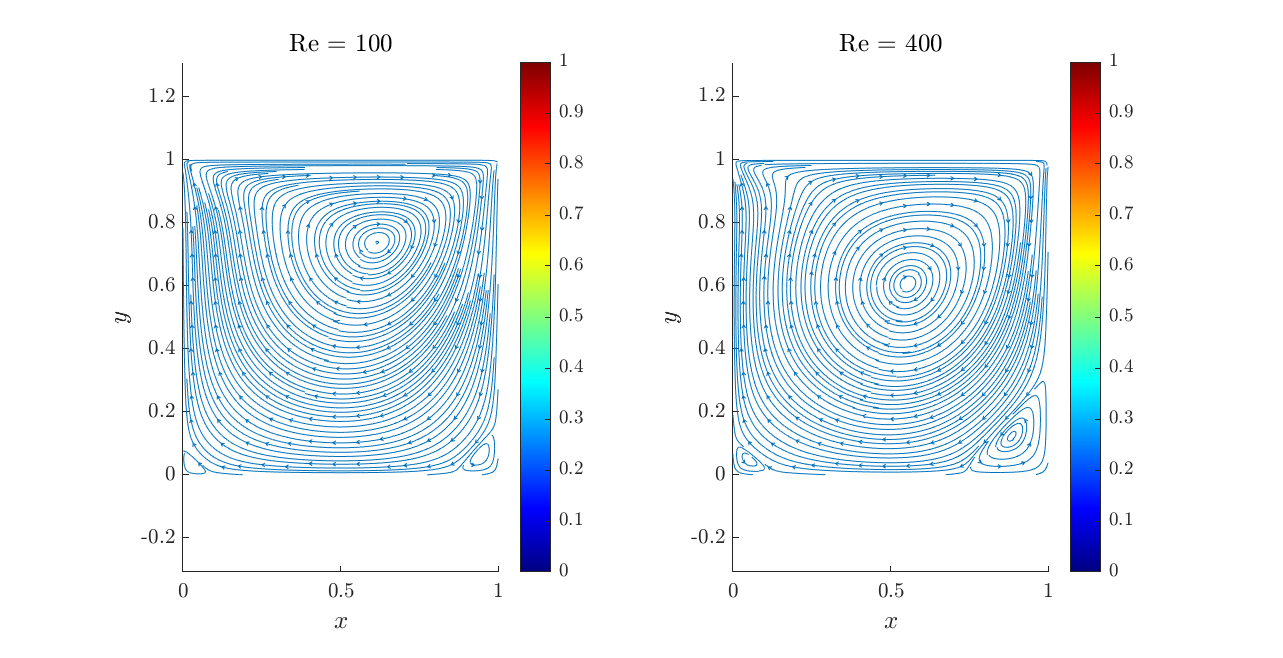
\includegraphics[trim=60 0 60 0, clip]{streamline.eps}
    \caption{$v$ Velocity Contours}
    \label{fig:v_velocity}
\end{figure}



\subsection{Convergence}
The residual error verses the number of iterations is plotted in post processing which is shown in  Fig.~\ref{}  for Re 100 and 400. The execution time and number of iterations executed for convergence are shown in Table~\ref{}.
\begin{figure}
    \centering
    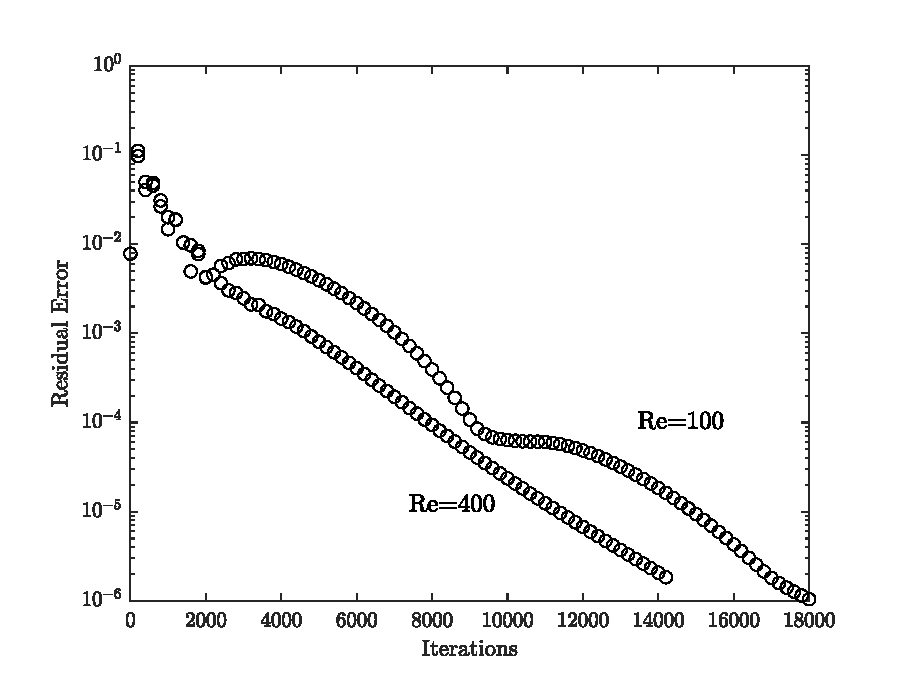
\includegraphics{residual.eps}
    \caption{$v$ Velocity Contours}
    \label{fig:v_velocity}
\end{figure}

\subsection{Contours}
\begin{figure}
    \centering
    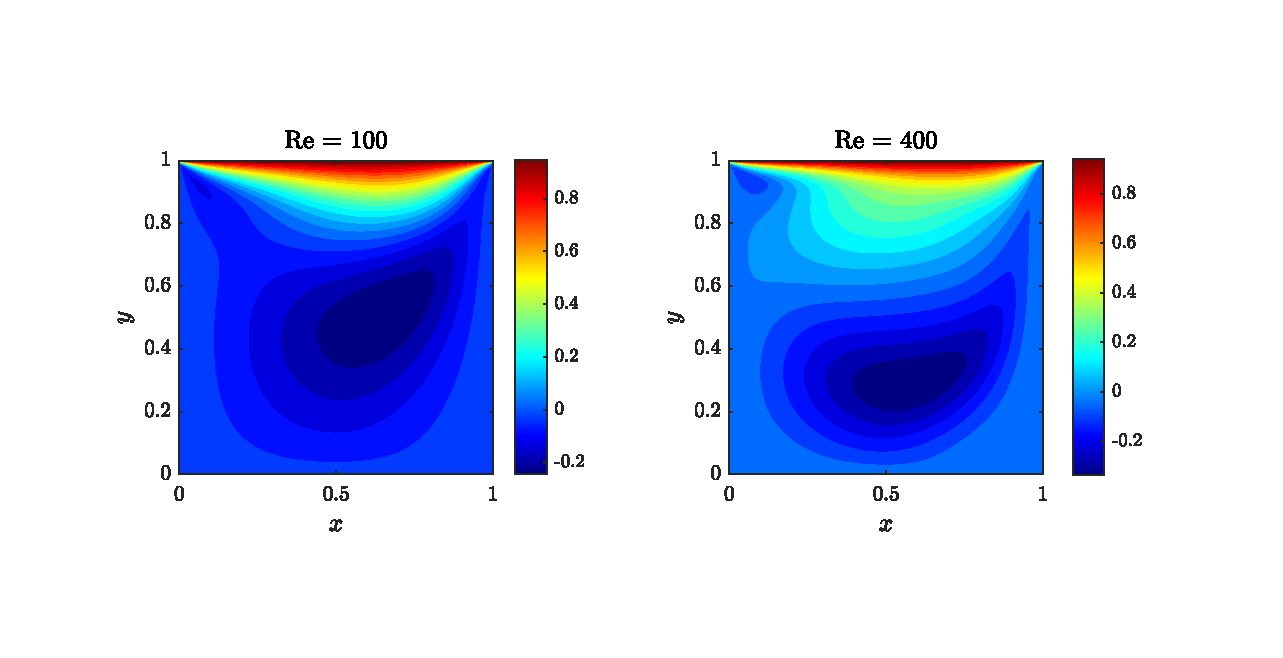
\includegraphics[trim=60 0 60 0, clip]{u_velocity.eps}
    \caption{u Velocity Contours}
    \label{fig:u_velocity}
\end{figure}
\begin{figure}
    \centering
    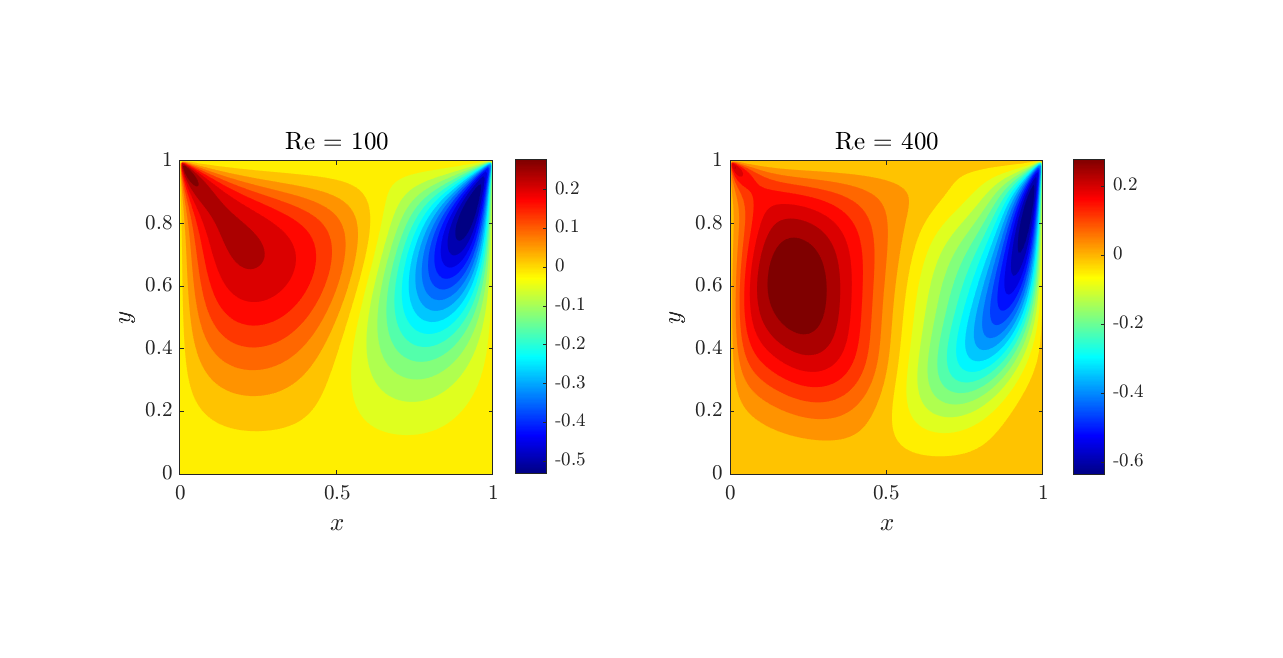
\includegraphics[trim=60 0 60 0, clip]{v_velocity.eps}
    \caption{$v$ Velocity Contours}
    \label{fig:v_velocity}
\end{figure}
\begin{figure}
    \centering
    \includegraphics[trim=60 0 60 0, clip]{stream_function.eps}
    \caption{$v$ Velocity Contours}
    \label{fig:v_velocity}
\end{figure}



\section{Conclusion}
In this project, the lid-driven cavity flow is solved using the SIMPLE method with varying Reynolds numbers. The velocity and streamline results are validated against the reference results from Ghia et al.~\cite{ghia1982high}. Grid size plays a crucial role in solution convergence and accuracy. Solving incompressible Navier-Stokes equations involves numerous intermediate steps, each of which must be computed carefully.

While solving the momentum equations, the convection term is discretized using the upwind method for velocity. Other methods, such as the QUICK scheme and the power-law scheme, offer higher accuracy and could be considered for further improvement. The Navier-Stokes momentum equations are solved implicitly, enabling larger time steps and potentially faster convergence rates. Solver performance and accuracy can be enhanced by employing these advanced methods. The time required to solve the pressure Poisson equation can be reduced by using sparse matrices and applying the Gauss elimination method to solve the pressure field efficiently. 

In summary, the lid-driven cavity flow serves as a benchmark test case for evaluating new computational fluid dynamics techniques due to its simple geometry and flow physics. In the future, I plan to work on solving the lid-driven cavity flow using the Fractional-Step Projection method, an implicit solver for incompressible and time-dependent Navier-Stokes equations.




















\end{document}
